% xelatex statestikz.tex
% or
% pdflatex statestikz.tex
% then
% pdf2svg statestikz.pdf statestikz.svg 1

\documentclass[border=2bp, tikz]{standalone}
\usepackage{tikz}

\usetikzlibrary{arrows,shapes.arrows,shapes.geometric,shapes.multipart,shapes.symbols}
\usetikzlibrary{calc}
\tikzset{
  state/.style={
    rectangle,
    draw=black, thick,
    minimum height=1.66em,
    text centered,
    rounded corners=3pt},
  branch/.style=
      {fill,shape=circle,minimum size=3pt,inner sep=0pt},
  cross line/.style={ preaction={draw=white, -, shorten >=2pt, shorten <=2pt, line width=2.5pt}},
}
\tikzset{>=latex}
%\usepackage{Baskervaldx}

\usepackage{fontspec}
\setmainfont{Petrona-Light}

\begin{document}
\begingroup
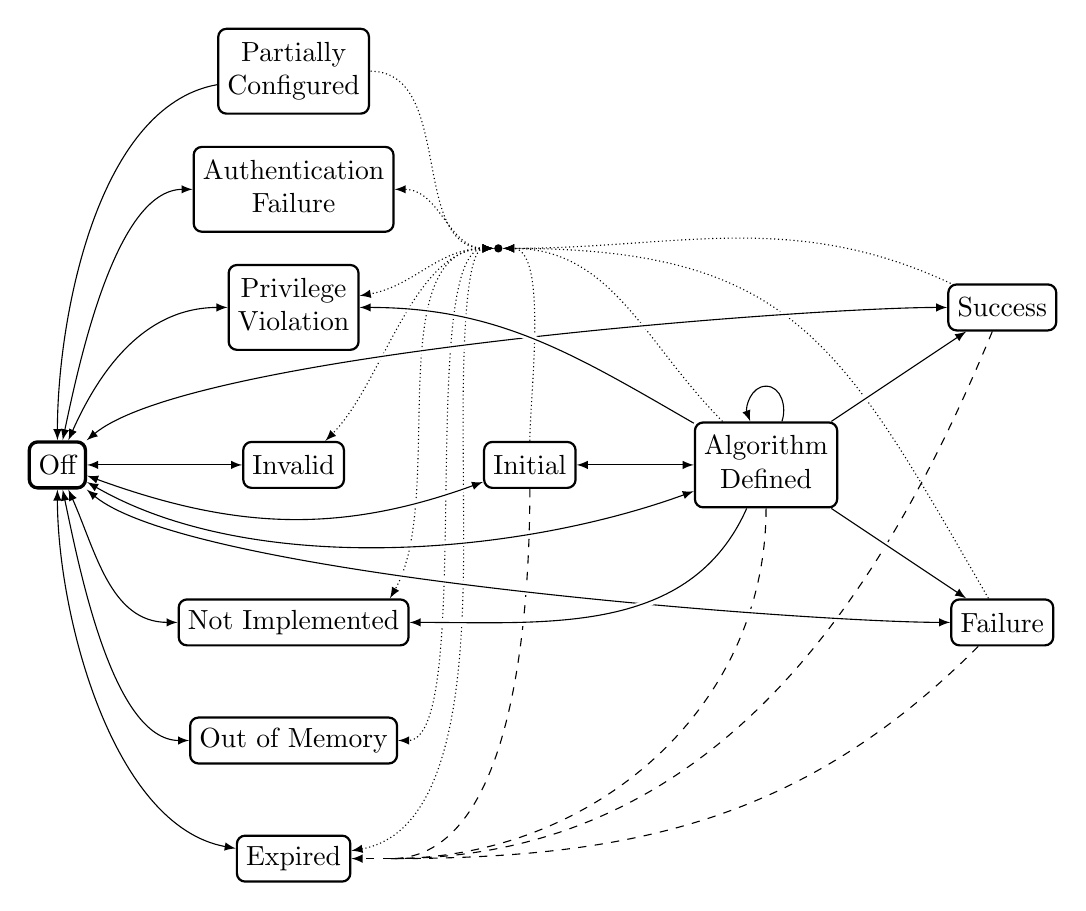
\begin{tikzpicture}
\node[state, very thick] at (0,0) (off)      {Off};

\node[state] at (3,0) (invalid)  {Invalid};
\node[state] at (3,-2) (NIMP)    {Not Implemented};
\node[state] at (3,-3.5) (OOM)     {Out of Memory};
\node[state] at (3,-5) (expired) {Expired};
\node[state] at (3,2) (privilege)  {\begin{tabular}{@{}c@{}}Privilege\\Violation\end{tabular}};
\node[state] at (3,3.5) (authfail)   {\begin{tabular}{@{}c@{}}Authentication\\Failure\end{tabular}};
\node[state] at (3,5) (partial)    {\begin{tabular}{@{}c@{}}Partially\\Configured\end{tabular}};

\node[branch] at (5.6,2.75) (joinsome) {};
\node[coordinate] at ($(expired.east)+(0.5,0)$) (jointoexpired) {};

\node[state] at (6,0) (initial)    {Initial};
\node[state] at (9,0) (algorithm)   {\begin{tabular}{@{}c@{}}Algorithm\\Defined\end{tabular}};
\node[state] at (12,2) (success)    {Success};
\node[state] at (12,-2) (failure)   {Failure};

\draw[->,densely dotted]  (initial) to[out=90,in=0,looseness=0.6] (joinsome);
\draw[->,densely dotted]  (algorithm)   to[out=135,in=0] (joinsome);
\draw[->,densely dotted]  (failure) to[out=120,in=0,looseness=1.25] (joinsome);
\draw[->,densely dotted]  (success) to[out=155,in=0] (joinsome);
\draw[<->,densely dotted] (joinsome) to[out=180,in=0] (authfail);
\draw[<-,densely dotted] (joinsome) to[out=180,in=0] (partial);
\draw[<->,densely dotted] (joinsome) to[out=180,in=10] (privilege);
\draw[<->,densely dotted] (joinsome) to[out=180,in=45,looseness=0.8] ($(invalid.north east)+(-0.25,0)$);
\draw[<->,densely dotted] (joinsome) to[out=180,in=60,looseness=0.8] ($(NIMP.north east)+(-0.25,0)$);
\draw[<->,densely dotted] (joinsome) to[out=180,in=0,looseness=0.4] (OOM);
\draw[<->,densely dotted] (joinsome) to[out=180,in=90,looseness=0.4] ($(initial.west)+(-0.25,0)$)
                                    to[out=270,in=10,looseness=0.8] ($(expired.east)+(0,0.1)$);

\draw[-,dashed]  (initial) to[out=270,in=0,looseness=0.8] (jointoexpired);
\draw[-,dashed]  (algorithm)   to[out=270,in=0] (jointoexpired);
\draw[-,dashed]  (success) to[out=247.5,in=0] (jointoexpired);
\draw[-,dashed]  (failure) to[out=225,in=0] (jointoexpired);
\draw[->,dashed]  (jointoexpired) -- (expired);


\draw[<->] (off) -- (invalid);
\draw[<-] (off) to[out=90,in=190,looseness=0.8] (partial);
\draw[<->] (off) to[out=78,in=180,looseness=0.7] (authfail);
\draw[<->] (off) to[out=66,in=180] (privilege);
\draw[<->] (off) to[out=294,in=180] (NIMP);
\draw[<->] (off) to[out=282,in=180,looseness=0.7] (OOM);
\draw[<->] (off) to[out=270,in=170,looseness=0.8] (expired);

\draw[<->,cross line] (off) to[out=-20,in=200] (initial);
\draw[<->,cross line] (off) to[out=-30,in=200,looseness=0.8] (algorithm);
\draw[<->,cross line] (off) to[out=40,in=180,looseness=0.4] (success);
\draw[<->,cross line] (off) to[out=-40,in=180,looseness=0.4] (failure);

\draw[<->] (initial) -- (algorithm);
%\draw[->, cross line] (initial) to[out=270,in=10] (expired);
%\draw[->, cross line] (initial) to[out=120,in=0] (privilege);

\draw[->,cross line] (algorithm) -- (success);
\draw[->,cross line] (algorithm) -- (failure);

\draw[->] (algorithm) to[out=70,in=0] ($(algorithm)+(0,1)$) to[out=180,in=110] (algorithm);
%\draw[->] (algorithm) to[out=160,in=20]  (invalid);
%\draw[->] (algorithm) to[out=270,in=0] (expired);
%\draw[->] (algorithm) to[out=258,in=0,looseness=0.7] (OOM);
\draw[->,cross line] (algorithm) to[out=246,in=0] (NIMP);
\draw[->,cross line] (algorithm) to[out=150,in=0] (privilege);
\end{tikzpicture}

\endgroup
\end{document}
